\documentclass{beamer}
\usepackage{verbatim}
\usepackage[english]{babel}
\usepackage{multirow}
\usepackage{graphicx}
\setbeamertemplate{caption}[numbered]
\usepackage{subcaption}
\usepackage{xcolor}
\usepackage{multirow}
\usepackage{algorithmicx}
\usepackage{algpseudocode}
\usepackage{comment}
\newcommand\figref{Figure~\ref}

\title{Singularity Graph Extraction}
\author{Continuous vs Discrete Strategies}
%\subtitle{Sample Subtitle}
\graphicspath{{img/}}
%\usetheme{lucid}
\begin{document}
	\frame {
		\titlepage
	}
	\begin{comment}
	\frame{
		\frametitle{Overall Algorithm Steps}
		 Given input mesh, 
		\begin{figure}[]
        \center{\includegraphics[width=10cm]
        {1}}
        \caption{Input triangular mesh}
      \end{figure}
		 %\includegraphics[height=7cm]{img/HIS-orig.png}
	}
	
	%%%%%%%%%%%%%%%%%%%%%%%%%%%%%%%%%%%%%%%%%%%%%%%%%%%%%%%%%%%%%%%%%%%%%%%%%%%%%%%%%%%%%%%%
	\frame{
		\frametitle{Overall Algorithm Steps}		
		\begin{itemize}
			\item 1. Construct Frame Field		
			
		\end{itemize}
		
		\begin{figure}[]
        \center{\includegraphics[width=10cm]
        {2}}
        \caption{Frame Field}
      \end{figure}
		%\includegraphics[height=7cm]{img/HIS-frame.png}
	}
	%%%%%%%%%%%%%%%%%%%%%%%%%%%%%%%%%%%%%%%%%%%%%%%%%%%%%%%%%%%%%%%%%%%%%%%%%%%%%%%%%%%%%%%%
	
	\frame{
		\frametitle{Overall Algorithm Steps}		
		\begin{itemize}
			\item 2. Construct Cross-Field (CF)			
			
		\end{itemize}
		\begin{figure}[]
        \center{\includegraphics[width=10cm]
        {HIS-frame-close-up.png}}
        \caption{Cross-Field - close-up}
      \end{figure}
		%\includegraphics[height=7cm]{img/HIS-frame-close-up.png}
	}
	
	%%%%%%%%%%%%%%%%%%%%%%%%%%%%%%%%%%%%%%%%%%%%%%%%%%%%%%%%%%%%%%%%%%%%%%%%%%%%%%%%%%%%%%%%
	\frame{
		\frametitle{Overall Algorithm Steps}		
		\begin{itemize}				
			\item 3. Trace separatrices of the CF
			
		\end{itemize}
		\begin{figure}[]
        \center{\includegraphics[width=10cm]
        {img/3}}
        \caption{Singularity Graph}
      \end{figure}
		%\includegraphics[height=7cm]{img/HIS-SingGraphOriginal-ConfusBallRad005.png}
	}
	
	%%%%%%%%%%%%%%%%%%%%%%%%%%%%%%%%%%%%%%%%%%%%%%%%%%%%%%%%%%%%%%%%%%%%%%%%%%%%%%%%%%%%%%%%
	\frame{
		\frametitle{Overall Algorithm Steps}	
		\begin{itemize}			
			\item 4. Remesh the resulted quad patches 
		\end{itemize}
		\begin{figure}[]
        \center{\includegraphics[width=10cm]
        {4}}
        \caption{Final quad mesh}
      \end{figure}
		%\includegraphics[height=7cm]{img/HIS-patches.png}
	}
	
	\end{comment}
	%%%%%%%%%%%%%%%%%%%%%%%%%%%%%%%%%%%%%%%%%%%%%%%%%%%%%%%%%%%%%%%%%%%%%%%%%%%%%%%%%%%%%%%%
	
	\frame {
		\frametitle{Trace separatrices of the CF}			
		%\[\frac{-b \pm \sqrt{b^2 - c}}{2a}\]		
		\begin{itemize}
			\item Detect the singular triangles and construct the singularity slots.
			\begin{figure}[]
        \center{\includegraphics[width=10cm]
        {SingZoom.png}}
        \caption{Singularities and slots (left - degree $3$, right - degree $5$)}
      \end{figure}
			%\includegraphics[height=7cm]{img/HIS-Slots.png}			
		\end{itemize}
	}
	%%%%%%%%%%%%%%%%%%%%%%%%%%%%%%%%%%%%%%%%%%%%%%%%%%%%%%%%%%%%%%%%%%%%%%%%%%%%%%%%%%%%%%%%
	%%%%%%%%%%%%%%%%%%%%%%%%%%%%%%%%%%%%%%%%%%%%%%%%%%%%%%%%%%%%%%%%%%%%%%%%%%%%%%%%%%%%%%%%
	\frame {
		\frametitle{Trace separatrices of the CF }			
		\framesubtitle{ Continuous Strategies}	
				(Iteratively/ Simultaneously) Depart from each singular point along each
slot direction until reaching:
\begin{itemize}
  \item[a)] the boundary
\newline
  \item[$b_1$)] the vicinity of a different singularity (confusing ball) - \textbf{Sequential Strategy} (Fig.~\ref{fig:seqStrat}).
\newline
  \item[$b_2$)] the vicinity of a different streamline (thresholdDistance) - \textbf{Simultaneous Strategy}	(Fig.~\ref{fig:simStrat}).	
\end{itemize}		
				
	}	
	
	%%%%%%%%%%%%%%%%%%%%%%%%%%%%%%%%%%%%%%%%%%%%%%%%%%%%%%%%%%%%%%%%%%%%%%%%%%%%%%%%%%%%%%%%
	\frame {
		\frametitle{Trace separatrices of the CF}
		\framesubtitle{ Continuous Strategies}
		 \begin{figure}[!ht]
            \centering
            \includegraphics[width=\textwidth]{HIS4-orig-Rad003}
            \caption{\small Sequential Strategy}  
            \label{fig:seqStrat}
        \end{figure}
	
	}
	%%%%%%%%%%%%%%%%%%%%%%%%%%%%%%%%%%%%%%%%%%%%%%%%%%%%%%%%%%%%%%%%%%%%%%%%%%%%%%%%%%%%%%%%
	%%%%%%%%%%%%%%%%%%%%%%%%%%%%%%%%%%%%%%%%%%%%%%%%%%%%%%%%%%%%%%%%%%%%%%%%%%%%%%%%%%%%%%%%
	\frame {
		\frametitle{Trace separatrices of the CF}
		\framesubtitle{ Continuous Strategies}
		 \begin{figure}[!hb]
            \centering
            \includegraphics[width=\textwidth]{HIS4-sim-Rad003}
            \caption{\small Simultaneous Strategy}
            \label{fig:simStrat}
        \end{figure}
	}
	
	%%%%%%%%%%%%%%%%%%%%%%%%%%%%%%%%%%%%%%%%%%%%%%%%%%%%%%%%%%%%%%%%%%%%%%%%%%%%%%%%%%%%%%%%
		\frame {
		\frametitle{Trace separatrices of the CF}
		\framesubtitle{ Continuous Strategies - Challenges}
		\begin{itemize}
	\item [$a)$] Dependence on input triangulation
	\item [$b)$] Dependence on proximity parameter 
      \begin{itemize}
       \item confusing ball radius - \textbf{Sequential Strategy} (Fig.~\ref{fig:seqStrat}).
       \item thresholdDistance - \textbf{Simultaneous Strategy}	(Fig.~\ref{fig:simStrat}).
      \end{itemize}
	  \end{itemize}		
	}
	%%%%%%%%%%%%%%%%%%%%%%%%%%%%%%%%%%%%%%%%%%%%%%%%%%%%%%%%%%%%%%%%%%%%%%%%%%%%%%%%%%%%%%%%
	%%%%%%%%%%%%%%%%%%%%%%%%%%%%%%%%%%%%%%%%%%%%%%%%%%%%%%%%%%%%%%%%%%%%%%%%%%%%%%%%%%%%%%%%
		\frame {
		\frametitle{Trace separatrices of the CF}
		\framesubtitle{ Continuous Strategies - Challenges}
	
	\begin{figure}[]
        \center{\includegraphics[width=8cm]
        {HIS4-sim-Rad002}}
        \caption{ "miss the connection"}
        \label{fig:figure4}
      \end{figure}	
			
	}
	%%%%%%%%%%%%%%%%%%%%%%%%%%%%%%%%%%%%%%%%%%%%%%%%%%%%%%%%%%%%%%%%%%%%%%%%%%%%%%%%%%%%%%%%
	%%%%%%%%%%%%%%%%%%%%%%%%%%%%%%%%%%%%%%%%%%%%%%%%%%%%%%%%%%%%%%%%%%%%%%%%%%%%%%%%%%%%%%%%
		\frame {
		\frametitle{Trace separatrices of the CF}
		\framesubtitle{ Continuous Strategies - Challenges}	
		%\framesubtitle{Algorithm Problems}
		%\ \center{A. Sequential Strategy}
	
	\begin{figure}[]
        \center{\includegraphics[width=7cm]
        {Circle_with_circle_holes_refSS1-cycle}}
        \caption{  Cycles}
        \label{fig:figure5}
      \end{figure}	
			
	}
	%%%%%%%%%%%%%%%%%%%%%%%%%%%%%%%%%%%%%%%%%%%%%%%%%%%%%%%%%%%%%%%%%%%%%%%%%%%%%%%%%%%%%%%%
	\begin{comment}
	\frame {
		\frametitle{Singularity Graph Building}		
		\framesubtitle{Algorithm Problems}
		%\[\frac{-b \pm \sqrt{b^2 - c}}{2a}\]
		\ \center{A. Sequential Strategy}
		\begin{columns}[T] % contents are top vertically aligned
     	\begin{column}[T]{5cm} % each column can also be its own environment
     	
     	\begin{figure}[]
        \center{\includegraphics[width=5cm]
        {img/HIS-SingGraphOriginal-ConfusBallRad001confusBall.png}}
        \caption{ Normal Radius}
      \end{figure}	
     	%\includegraphics[height=3.7cm]{img/HIS-SingGraphOriginal-ConfusBallRad001confusBall.png}
     	\end{column}
     	\begin{column}[T]{5cm} % alternative top-align that's better for graphics
     	 
     	\begin{figure}[]
        \center{\includegraphics[width=5cm]
        {img/HIS-SingGraphOriginal-ConfusBallRad005confusBall.png}}
        \caption{ Big Radius}
      \end{figure}	
          %\includegraphics[height=3.7cm]{img/HIS-SingGraphOriginal-ConfusBallRad005confusBall.png}
     	\end{column}
     	\end{columns}
			
	}
	\end{comment}
	%%%%%%%%%%%%%%%%%%%%%%%%%%%%%%%%%%%%%%%%%%%%%%%%%%%%%%%%%%%%%%%%%%%%%%%%%%%%%%%%%%%%%%%%
		\frame {
		\frametitle{Trace separatrices of the CF - Discrete Strategy}			
		\framesubtitle{ }	
		\begin{itemize}
		 \item Build a connectivity graph $G$ from $T$ %of shortest paths, using a modified Dijkstra's algorithm.
		 \item Compute shortest paths between slots on $G \rightarrow {SP}_G \subset G$
		 \item Extract from ${SP_G}$ the expected singularity graph
		\end{itemize}				
				
\textbf{Advantages}
\begin{itemize}
 \item No infinite cycles.
 \item More possible connections - a matter of choice.
\end{itemize}

\textbf{Limitations}
\begin{itemize}
 \item Depends on the mesh resolution.
 \item Computationally expensive.
\end{itemize}
				
	}

	
	%%%%%%%%%%%%%%%%%%%%%%%%%%%%%%%%%%%%%%%%%%%%%%%%%%%%%%%%%%%%%%%%%%%%%%%%%%%%%%%%%%%%%%%%
			
		
		
		\frame {
	\frametitle{Discrete Strategy }			
		\framesubtitle{Build a connectivity graph $G = (V, E)$ from $T$}		
	\begin{itemize}
		 \item A vertex $v$ of $V$ is a triangle of $T$ %of shortest paths, using a modified Dijkstra's algorithm.
		 \item An edge $e$ of $E$ (a path) links to two vertices corresponding to two triangles of $T$ sharing at least a node
		 \item First, detect slot vertices $S_v \subset V$
		 \item Using RK4 integration, we get one triangle of $T$ per slot - triangles that do not share any vertex by construction
		\end{itemize}		
		
	\begin{figure}[]
        \center{\includegraphics[width=4.5cm]
        {img1}}
        \caption{ Neighbouring triangles by node}
        \label{fig:figure6}
      \end{figure}	
			
	}
	
	
	%%%%%%%%%%%%%%%%%%%%%%%%%%%%%%%%%%%%%%%%%%%%%%%%%%%%%%%%%%%%%%%%%%%%%%%%%%%%%%%%%%%%%%%%
			
		
		
		\frame {
	\frametitle{Discrete Strategy }			
	\framesubtitle{Build the slot-connectivity graph $S_G = (V_G, E_G)$}		
	\begin{itemize}
		 \item All slot vertices are in the connectivity graph $ \rightarrow S_v \subseteq S_G$ 
		 \item Edges of $E_G$ are built as shortest paths from a vertex of $S_v$ towards a vertex of $S_v \cap S_{bnd}$
		 \begin{itemize}
		 	\item Dijkstra-like algorithm from each vertex of $S_v$ until reaching all the other vertices of $S_v$ and (at least) one vertex of $S_{bnd}$
		\end{itemize}		
	\end{itemize}		
		
	\begin{figure}[]
        \center{\includegraphics[width=6cm]{img2}}
        \caption{ From each slot depart towards all other slots}
        \label{fig:figure7}
      \end{figure}	
			
	}
%%%%%%%%%%%%%%%%%%%%%%%%%%%%%%%%%%%%%%%%%%%%%%%%%%%%%%%%%%%%%%%%%%%%%%%%%%%%%%%%%%%%%%%%
			
\frame {
	\frametitle{Discrete Strategy }			
	\framesubtitle{Build the slot-connectivity graph $S_G = (V_G, E_G)$ }		
	\begin{itemize}
		 \item Edge weight during Dijkstra-like traversal: $\omega_{\angle(c_i, c_j)} + (\alpha_i + \alpha_j)$ 	
		 \begin{itemize}
		 	\item $\alpha_i $ and $ \alpha_j \rightarrow $ edge deviation to the cross field
			\item $c_i$ depends on the incoming vertex (previous edge)
			\item $\omega_{\angle(c_i, c_j)} = 1$ if $\sphericalangle{(c_i, c_j)} < \pi/4$
			\item $\omega_{\angle(c_i, c_j)} = \infty$ otherwise
		 \end{itemize}
	\end{itemize}
		
	\begin{figure}[]
        \center{\includegraphics[width=6cm]{img3}}
        \caption{ Edge	weight illustration}
        \label{fig:figure8}
    \end{figure}		
			
}
%%%%%%%%%%%%%%%%%%%%%%%%%%%%%%%%%%%%%%%%%%%%%%%%%%%%%%%%%%%%%%%%%%%%%%%%%%%%%%%%%%%%%%%%	
	\frame {
	\frametitle{Discrete Strategy }			
		\framesubtitle{Extract the	singularity graph	from  $S_G = (V_G, E_G)$ }	
		 Too many edges in $E_G$ %- \figref{fig:img5}	
		
	\begin{figure}[]
        \center{\includegraphics[width=6cm]{img5}}
        \caption{Slot-connectivity graph - the entire set of paths}
        \label{fig:figure9}
      \end{figure}				
	}
	
	%%%%%%%%%%%%%%%%%%%%%%%%%%%%%%%%%%%%%%%%%%%%%%%%%%%%%%%%%%%%%%%%%%%%%%%%%%%%%%%%%%%%%%%%	
	\frame {
	\frametitle{Discrete Strategy }			
		\framesubtitle{Extract the	singularity graph	from  $S_G = (V_G, E_G)$ }	
		 Objectives
	\begin{itemize}
		 \item Keep exactly only edge per slot of $S_G$ 
		  \item Ideally, shortest edge must be kept (best cross field follower)
		  \item  Constraint between incompatible edges of $E_G$ (keep at most one)
		 \begin{itemize}
		 	\item Yellow and blue paths follow the same direction locally  %\figref{fig:img4}	 
		\end{itemize}
	\end{itemize}		
		
	\begin{figure}[]
        \center{\includegraphics[width=6cm]{img4}}
        \caption{Incompatible paths}
        \label{fig:figure10}
      \end{figure}				
	}
	%%%%%%%%%%%%%%%%%%%%%%%%%%%%%%%%%%%%%%%%%%%%%%%%%%%%%%%%%%%%%%%%%%%%%%%%%%%%%%%%%%%%%%%%
	\frame {
	\frametitle{Discrete Strategy }
		\framesubtitle{Extract the singularity graph from  $S_G = (V_G, E_G)$ }
		Optimization $\rightarrow min \sum_i \omega_i * p_i$, such that: 
	\begin{itemize}
	     \item Variables $p_i$ are integer $(1 -$ keep edge $e_i$, $0 - $ discard edge $)$ $\rightarrow$ \textcircled{1}$ \forall i \in I, p_i \in \{0;1\} $
		 \item Keep exactly one edge per slot of $S_G$ $\rightarrow$ \textcircled{2} $\forall s \in {slots}, \sum_{e\in{Adj(s)}} e = 1$
		  \item Ideally, shortest edge must be kept (best cross field follower) $\rightarrow$ weight $\omega$ in the objective function.
		  \item  Constraint between incompatible edges of $E_G$ $\rightarrow$ \textcircled{3} $\forall (p_i, p_j) \in C, p_i + p_j \leq 1$  
		\end{itemize}
	}
%%%%%%%%%%%%%%%%%%%%%%%%%%%%%%%%%%%%%%%%%%%%%%%%%%%%%%%%%%%%%%%%%%%%%%%%%%%%%%%%%%%%%%%%
%%%%%%%%%%%%%%%%%%%%%%%%%%%%%%%%%%%%%%%%%%%%%%%%%%%%%%%%%%%%%%%%%%%%%%%%%%%%%%%%%%%%%%%%
\begin{comment}
		\frame {
	\frametitle{Trace separatrices of the CF }			
		\framesubtitle{2. Discrete Strategy}		
	
	\begin{figure}[]
        \center{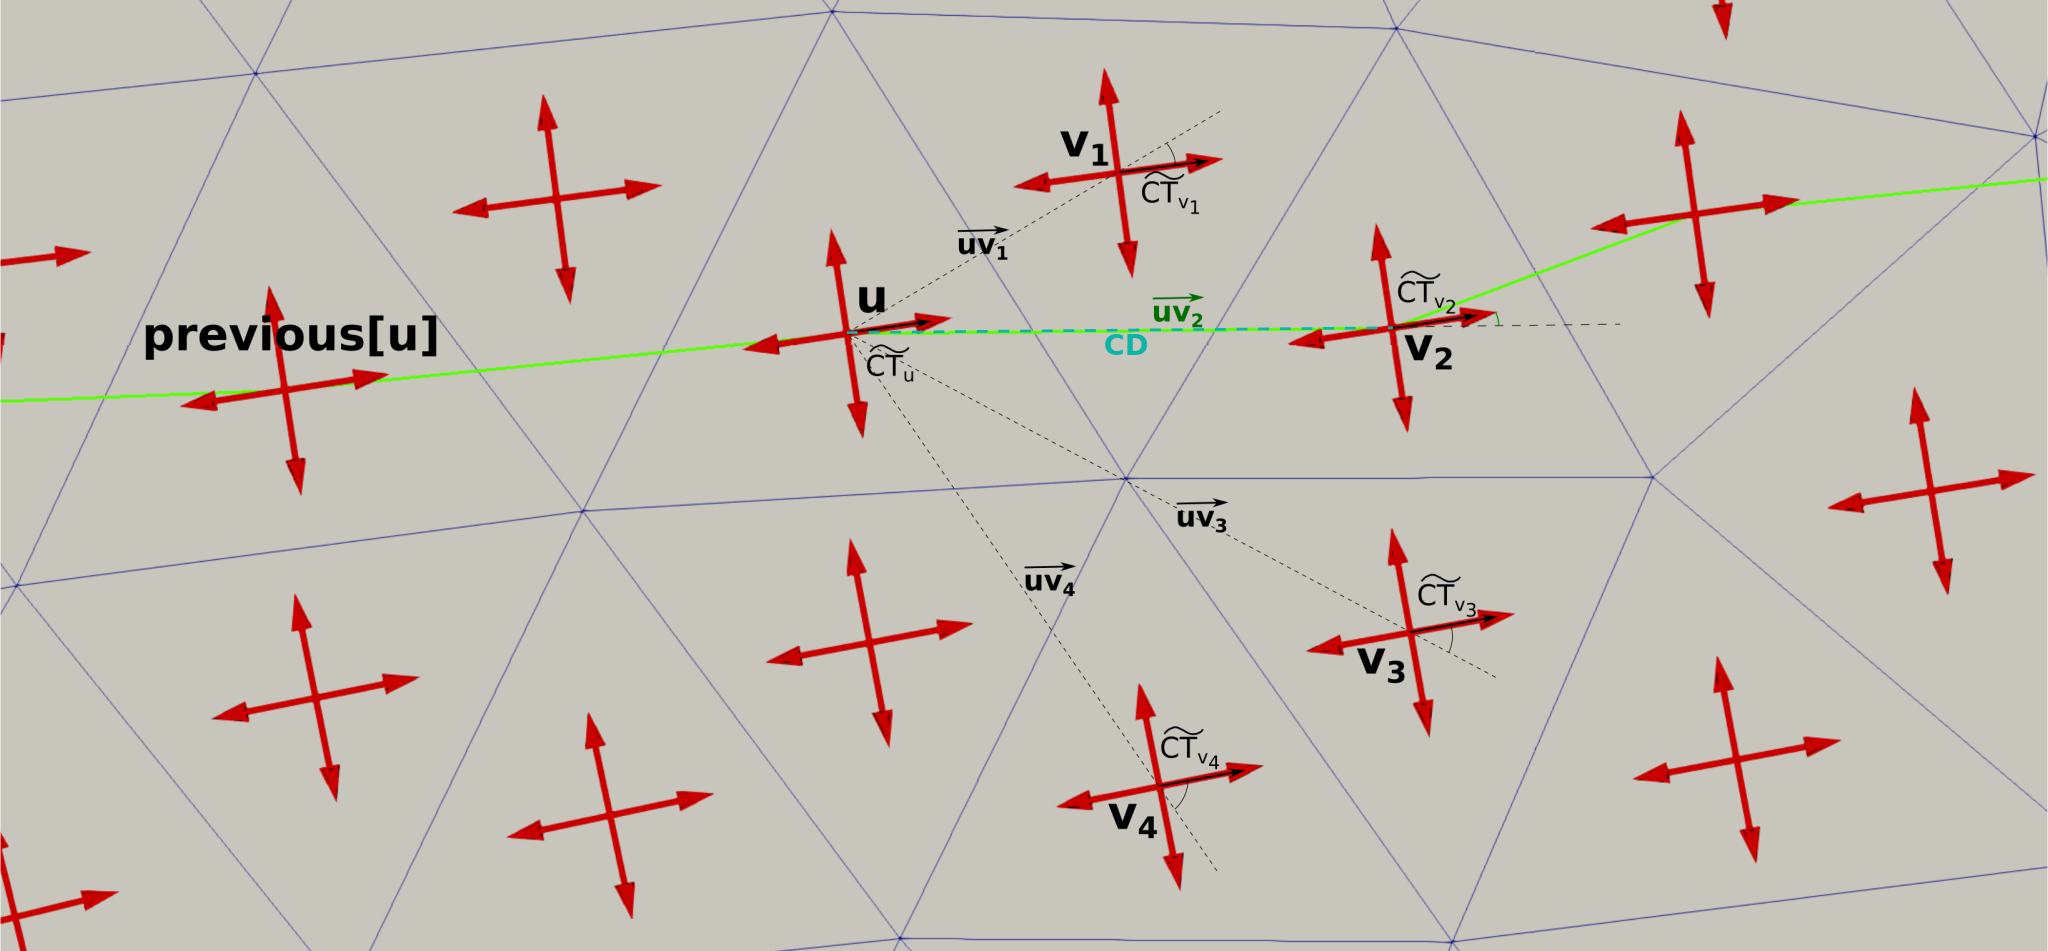
\includegraphics[width=8cm]
        {shortestPaths-zoom2}}
        \caption{ Discrete Strategy - Algorithm description}
        %\label{fig:figure9}
      \end{figure}	
			
	}
	
		%%%%%%%%%%%%%%%%%%%%%%%%%%%%%%%%%%%%%%%%%%%%%%%%%%%%%%%%%%%%%%%%%%%%%%%%%%%%%%%%%%%%%%%%
		\frame {
	\frametitle{Trace separatrices of the CF }			
		\framesubtitle{2. Discrete Strategy}		
	\begin{itemize}
	 \item Starting from a triangle slot - $source$
	 \item Walk along triangle centers $(u, v_0, v_1...)$, visiting adjacent triangles $(Neigh)$	
	 \item Distance as the angle difference between the (previous and current ) crosses and between the geometric direction ($\overrightarrow{uv}$) and the previous cross
	 \item Get the shortest paths towards the slots of other singularities (or boundary) - $Targets$
	\end{itemize}	
			
	}
\end{comment}
		%%%%%%%%%%%%%%%%%%%%%%%%%%%%%%%%%%%%%%%%%%%%%%%%%%%%%%%%%%%%%%%%%%%%%%%%%%%%%%%%%%%%%%%%
\begin{comment}
		\frame {
		\frametitle{Trace separatrices of the CF }			
		\framesubtitle{2. Discrete Strategy - Algorithm Shortest Paths}		

		\begin{algorithmic}[1]
		\State $d[source]\gets 0$
		\While{$Q\not=\emptyset$}
		\State $u:= center\ of\ triangle\ in\ Q$
		\State $Q\gets Q\setminus u$
		\If{$u\in Targets$}
		\State{$d[u] = d[u] + w\_pen * \angle(CT_{previous}[u] -CT_{target\_slot\_u})$}
		\State{$return\ u$}
		\EndIf
		\For{$v\in Neigh(u); v\ not\ visited$}
		\State $\widetilde{CT_v}\gets closest\ {CT_v}\ w.r.t\ \widetilde{CT_u}$
		\State $d_{temp}\gets d[u] + w\_pen * \angle(\widetilde{CT_u}, \widetilde{CT_v}) + 		\angle(\widetilde{CT_v}, \overrightarrow{uv})$
		\If{$d_{temp} < d[v]$}
		\State $d[v]\gets d_{temp}$
		\State $previous[v] = u$
		\State $CT_{previous}[v] = \widetilde{CT_v}$
		\EndIf
		\EndFor
		\EndWhile
		\end{algorithmic}				
	}	
		%%%%%%%%%%%%%%%%%%%%%%%%%%%%%%%%%%%%%%%%%%%%%%%%%%%%%%%%%%%%%%%%%%%%%%%%%%%%%%%%%%%%%%%%
		
	\frame {
	\frametitle{Trace separatrices of the CF }			
	\framesubtitle{2. Discrete Strategy}		
	\begin{itemize}
	 \item For each slot (singular or geometric slot) compute the shortest path towards all other 	slots (excluding slots belonging to the same singularity) and boundary	 
	 \begin{itemize}
	 \item[•] only connections for which the deviation 
	 \end{itemize}
	 \item Walk along triangle centers $(u, v_0, v_1...)$, visiting adjacent triangles $(Neigh)$	
	 \item Distance as the angle difference between the (previous and current ) crosses and 		between the geometric direction ($\overrightarrow{uv}$) and the previous cross
	 \item Get the shortest paths towards the slots of other singularities (or boundary) - 		$Targets$
	\end{itemize}	
			
	}
	%%%%%%%%%%%%%%%%%%%%%%%%%%%%%%%%%%%%%%%%%%%%%%%%%%%%%%%%%%%%%%%%%%%%%%%%%%%%%%%%%%%%%%%%		
	\frame {
	\frametitle{Trace separatrices of the CF }			
	\framesubtitle{2. Discrete Strategy}		
	\begin{itemize}
	 \item Starting from a triangle slot - $source$
	 \item Walk along triangle centers $(u, v_0, v_1...)$, visiting adjacent triangles $(Neigh)$	
	 \item Distance as the angle difference between the (previous and current ) crosses and between the geometric direction ($\overrightarrow{uv}$) and the previous cross
	 \item Get the shortest paths towards the slots of other singularities (or boundary) - $Targets$
	\end{itemize}	
			
	}
	%%%%%%%%%%%%%%%%%%%%%%%%%%%%%%%%%%%%%%%%%%%%%%%%%%%%%%%%%%%%%%%%%%%%%%%%%%%%%%%%%%%%%%%%	
	\frame {
	\frametitle{Trace separatrices of the CF }			
		\framesubtitle{2. Discrete Strategy}		
	\begin{itemize}
	 \item Starting from a triangle slot - $source$
	 \item Walk along triangle centers $(u, v_0, v_1...)$, visiting adjacent triangles $(Neigh)$	
	 \item Distance as the angle difference between the (previous and current ) crosses and between the geometric direction ($\overrightarrow{uv}$) and the previous cross
	 \item Get the shortest paths towards the slots of other singularities (or boundary) - $Targets$
	\end{itemize}	
			
	}
	%%%%%%%%%%%%%%%%%%%%%%%%%%%%%%%%%%%%%%%%%%%%%%%%%%%%%%%%%%%%%%%%%%%%%%%%%%%%%%%%%%%%%%%%	
	\frame {
	\frametitle{Trace separatrices of the CF }			
		\framesubtitle{2. Discrete Strategy}		
	\begin{itemize}
	 \item Starting from a triangle slot - $source$
	 \item Walk along triangle centers $(u, v_0, v_1...)$, visiting adjacent triangles $(Neigh)$	
	 \item Distance as the angle difference between the (previous and current ) crosses and between the geometric direction ($\overrightarrow{uv}$) and the previous cross
	 \item Get the shortest paths towards the slots of other singularities (or boundary) - $Targets$
	\end{itemize}	
			
	}
	%%%%%%%%%%%%%%%%%%%%%%%%%%%%%%%%%%%%%%%%%%%%%%%%%%%%%%%%%%%%%%%%%%%%%%%%%%%%%%%%%%%%%%%%	
	\frame {
	\frametitle{Trace separatrices of the CF }			
		\framesubtitle{2. Discrete Strategy}		
	\begin{itemize}
	 \item Starting from a triangle slot - $source$
	 \item Walk along triangle centers $(u, v_0, v_1...)$, visiting adjacent triangles $(Neigh)$	
	 \item Distance as the angle difference between the (previous and current ) crosses and between the geometric direction ($\overrightarrow{uv}$) and the previous cross
	 \item Get the shortest paths towards the slots of other singularities (or boundary) - $Targets$
	\end{itemize}	
			
	}		
	%%%%%%%%%%%%%%%%%%%%%%%%%%%%%%%%%%%%%%%%%%%%%%%%%%%%%%%%%%%%%%%%%%%%%%%%%%%%%%%%%%%%%%%%
		
	\frame {
	\frametitle{Trace separatrices of the CF - Discrete Strategy}		
	
	\begin{figure}[]
        \center{\includegraphics[width=8cm]
        {HIS3-shortest_paths}}
        \caption{ Discrete Strategy - $|T| = 7219$}
        %\label{fig:figure9}
      \end{figure}	
			
	}
		%%%%%%%%%%%%%%%%%%%%%%%%%%%%%%%%%%%%%%%%%%%%%%%%%%%%%%%%%%%%%%%%%%%%%%%%%%%%%%%%%%%%%%%%
	
	\frame {
	\frametitle{Trace separatrices of the CF - Discrete Strategy}		
	
	\begin{figure}[]
        \center{\includegraphics[width=8cm]
        {HIS6-shortest_paths}}
        \caption{ Discrete Strategy - $|T| = 102707$}
        %\label{fig:figure9}
      \end{figure}	
			
	}
\end{comment}
	%%%%%%%%%%%%%%%%%%%%%%%%%%%%%%%%%%%%%%%%%%%%%%%%%%%%%%%%%%%%%%%%%%%%%%%%%%%%%%%%%%%%%%%%
		
	\frame {
	\frametitle{Trace separatrices of the CF - Discrete Strategy}		
	
	\begin{figure}[]
        \center{\includegraphics[width=7cm]
        {Circle_with_circle_holes_ref_graph}}
        \caption{ Discrete Strategy - No cycles ($CWCH\_ref$)}
        \label{fig:figure11}
      \end{figure}	
			
	}

	%%%%%%%%%%%%%%%%%%%%%%%%%%%%%%%%%%%%%%%%%%%%%%%%%%%%%%%%%%%%%%%%%%%%%%%%%%%%%%%%%%%%%%%%
	
	
	\frame {
\frametitle{Trace separatrices of the CF - Discrete Strategy}		
	
	\begin{figure}[]
        \center{\includegraphics[width=7cm]
        {Circle_with_circle_holes_coarse_graph}}
        \caption{ Discrete Strategy - No cycles ($CWCH\_coarse$)}
        %\label{fig:figure9}
      \end{figure}	
			
	}

%%%%%%%%%%%%%%%%%%%%%%%%%%%%%%%%%%%%%%%%%%%%%%%%%%%%%%%%%%%%%%%%%%%%%%%%%%%%%%%%%%%%%%%%
	
	\frame {
\frametitle{Trace separatrices of the CF - Discrete Strategy}		
	- increasing mesh resolution will result in a higher fidelity of the paths founds w.r.t. the field
	\begin{figure}[]
        \center{\includegraphics[width=7cm]
        {HIS0_graph}}
        \caption{Mesh $HIS_{0}$}
        %\label{fig:figure9}
      \end{figure}	
			
	}
	
	
	\frame {
\frametitle{Trace separatrices of the CF - Discrete Strategy}		
	- increasing mesh resolution will result in a higher fidelity of the paths founds w.r.t. the field
	\begin{figure}[]
        \center{\includegraphics[width=7cm]
        {HIS2_graph}}
        \caption{Mesh $HIS_{2}$}
        %\label{fig:figure9}
      \end{figure}	
			
	}
	
	
	\frame {
\frametitle{Trace separatrices of the CF - Discrete Strategy}	
	- increasing mesh resolution will result in a higher fidelity of the paths founds w.r.t. the field
	\begin{figure}[]
        \center{\includegraphics[width=7cm]
        {HIS3_graph}}
        \caption{Mesh $HIS_{3}$}
        %\label{fig:figure9}
      \end{figure}	
			
	}
	
	
	
	\frame {
\frametitle{Trace separatrices of the CF - Discrete Strategy}		
	- increasing mesh resolution will result in a higher fidelity of the paths founds w.r.t. the field
	\begin{figure}[]
        \center{\includegraphics[width=7cm]
        {HIS4_graph}}
        \caption{Mesh $HIS_{4}$}
        %\label{fig:figure9}
      \end{figure}	
			
	}
	
	
	
	\frame {
\frametitle{Trace separatrices of the CF - Discrete Strategy}		
	- increasing mesh resolution will result in a higher fidelity of the paths founds w.r.t. the field
	\begin{figure}[]
        \center{\includegraphics[width=7cm]
        {HIS5_graph}}
        \caption{Mesh $HIS_{5}$}
        %\label{fig:figure9}
      \end{figure}	
			
	}
	
	
	
	\frame {
\frametitle{Trace separatrices of the CF - Discrete Strategy}		
	- increasing mesh resolution will result in a higher fidelity of the paths founds w.r.t. the field
	\begin{figure}[]
        \center{\includegraphics[width=7cm]
        {HIS6_graph}}
        \caption{Mesh $HIS_{6}$}
        %\label{fig:figure9}
      \end{figure}	
			
	}
	
	%%%%%%%%%%%%%%%%%%%%%%%%%%%%%%%%%%%%%%%%%%%%%%%%%%%%%%%%%%%%%%%%%%%%%%%%%%%%%%%%%%%%%%%%
	\frame {
\frametitle{Trace separatrices of the CF - Discrete Strategy}		
	
	\begin{figure}[]
     	\begin{subfigure}{\linewidth}
  \includegraphics[width=.22\linewidth]
  {E_graph}\hfill
  \includegraphics[width=.22\linewidth]
  {D2_graph}\hfill
  \includegraphics[width=.22\linewidth]
  {D3_graph}\hfill
  \end{subfigure}\par\medskip
        \caption{Mesh $E$, Mesh $D_2$ and Mesh $D_3$}
      \end{figure}
			
	}
	
	%%%%%%%%%%%%%%%%%%%%%%%%%%%%%%%%%%%%%%%%%%%%%%%%%%%%%%%%%%%%%%%%%%%%%%%%%%%%%%%%%%%%%%%%
	\begin{comment}
	\frame {
\frametitle{Trace separatrices of the CF - Discrete Strategy}		
	
	
      \begin{figure}[]
        \center{\includegraphics[width=5cm]
        {E_graph}}
        \caption{Mesh $E$}
        %\label{fig:figure9}
      \end{figure}	
			
	}
	
	
	
		%%%%%%%%%%%%%%%%%%%%%%%%%%%%%%%%%%%%%%%%%%%%%%%%%%%%%%%%%%%%%%%%%%%%%%%%%%%%%%%%%%%%%%%%
	
	\frame {
\frametitle{Trace separatrices of the CF - Discrete Strategy}		
	
	\begin{figure}[]
        \center{\includegraphics[width=7cm]
        {E_graph}}
        \caption{Mesh $E$}
        %\label{fig:figure9}
      \end{figure}	
			
	}
	

	
	%%%%%%%%%%%%%%%%%%%%%%%%%%%%%%%%%%%%%%%%%%%%%%%%%%%%%%%%%%%%%%%%%%%%%%%%%%%%%%%%%%%%%%%%
	
	\frame {
\frametitle{Trace separatrices of the CF - Discrete Strategy}		
	
	\begin{figure}[]
        \center{\includegraphics[width=7cm]
        {D2_graph}}
        \caption{Mesh $D_2$}
        %\label{fig:figure9}
      \end{figure}	
			
	}
	
	%%%%%%%%%%%%%%%%%%%%%%%%%%%%%%%%%%%%%%%%%%%%%%%%%%%%%%%%%%%%%%%%%%%%%%%%%%%%%%%%%%%%%%%%
	
	\frame {
\frametitle{Trace separatrices of the CF - Discrete Strategy}		
	
	\begin{figure}[]
        \center{\includegraphics[width=7cm]
        {D3_graph}}
        \caption{Mesh $D_3$}
        %\label{fig:figure9}
      \end{figure}	
			
	}
	\end{comment}
	%%%%%%%%%%%%%%%%%%%%%%%%%%%%%%%%%%%%%%%%%%%%%%%%%%%%%%%%%%%%%%%%%%%%%%%%%%%%%%%%%%%%%%%%
	\begin{comment}
	\begin{figure}[]
        \center{\includegraphics[width=5cm]
        {C_graph}}
        \caption{Mesh $C$}
        %\label{fig:figure9}
      \end{figure}	
		
	
	\frame {
\frametitle{Trace separatrices of the CF - Discrete Strategy}		
	
	\begin{figure}[]
        \center{\includegraphics[width=7cm]
        {F_graph}}
        \caption{Mesh $F$}
        %\label{fig:figure9}
      \end{figure}	
			
	}
	
	%%%%%%%%%%%%%%%%%%%%%%%%%%%%%%%%%%%%%%%%%%%%%%%%%%%%%%%%%%%%%%%%%%%%%%%%%%%%%%%%%%%%%%%%
	\frame {
\frametitle{Trace separatrices of the CF - Discrete Strategy}		
	
	\begin{figure}[]
        \center{\includegraphics[width=7cm]
        {F2_graph}}
        \caption{Mesh $F_2$}
        %\label{fig:figure9}
      \end{figure}	
			
	}
	\end{comment}
	
	%%%%%%%%%%%%%%%%%%%%%%%%%%%%%%%%%%%%%%%%%%%%%%%%%%%%%%%%%%%%%%%%%%%%%%%%%%%%%%%%%%%%%%%%
	
	\frame {
\frametitle{Trace separatrices of the CF - Discrete Strategy}		
	
	\begin{figure}[]
     	\begin{subfigure}{\linewidth}
  \includegraphics[width=.45\linewidth]
  {L_01_graph}\hfill
  \includegraphics[width=.45\linewidth]
  {L_04_graph}\hfill
  \end{subfigure}\par\medskip
        \caption{Mesh $L_{01}$ and Mesh $L_{04}$}
      \end{figure}
			
	}
	
	%%%%%%%%%%%%%%%%%%%%%%%%%%%%%%%%%%%%%%%%%%%%%%%%%%%%%%%%%%%%%%%%%%%%%%%%%%%%%%%%%%%%%%%%
	
	\frame {
\frametitle{Trace separatrices of the CF - Discrete Strategy}		
	
	\begin{figure}[]
     	\begin{subfigure}{\linewidth}
  \includegraphics[width=.45\linewidth]
  {M_04_graph}\hfill
  \includegraphics[width=.45\linewidth]
  {M_07_graph}\hfill
  \end{subfigure}\par\medskip
        \caption{Mesh $M_{04}$ and Mesh $M_{07}$}
      \end{figure}
			
	}
	%%%%%%%%%%%%%%%%%%%%%%%%%%%%%%%%%%%%%%%%%%%%%%%%%%%%%%%%%%%%%%%%%%%%%%%%%%%%%%%%%%%%%%%%
	
	\begin{comment}
	\frame {
\frametitle{Trace separatrices of the CF - Discrete Strategy}		
	
	\begin{figure}[]
        \center{\includegraphics[width=7cm]
        {L_01_graph}}
        \caption{Mesh $L_01$}
        %\label{fig:figure9}
      \end{figure}	
			
	}
	
	%%%%%%%%%%%%%%%%%%%%%%%%%%%%%%%%%%%%%%%%%%%%%%%%%%%%%%%%%%%%%%%%%%%%%%%%%%%%%%%%%%%%%%%%
	
	
	\frame {
\frametitle{Trace separatrices of the CF - Discrete Strategy}		
	
	\begin{figure}[]
        \center{\includegraphics[width=7cm]
        {L_04_graph}}
        \caption{Mesh $L_04$}
        %\label{fig:figure9}
      \end{figure}	
			
	}
	
	%%%%%%%%%%%%%%%%%%%%%%%%%%%%%%%%%%%%%%%%%%%%%%%%%%%%%%%%%%%%%%%%%%%%%%%%%%%%%%%%%%%%%%%%
	
	
	\frame {
\frametitle{Trace separatrices of the CF - Discrete Strategy}		
	
	\begin{figure}[]
        \center{\includegraphics[width=7cm]
        {M_04_graph}}
        \caption{Mesh $M_{04}$}
        %\label{fig:figure9}
      \end{figure}	
			
	}	
	
	%%%%%%%%%%%%%%%%%%%%%%%%%%%%%%%%%%%%%%%%%%%%%%%%%%%%%%%%%%%%%%%%%%%%%%%%%%%%%%%%%%%%%%%%
	
	
	\frame {
\frametitle{Trace separatrices of the CF - Discrete Strategy}		
	
	\begin{figure}[]
        \center{\includegraphics[width=7cm]
        {M_07_graph}}
        \caption{Mesh $M_{07}$}
        %\label{fig:figure9}
      \end{figure}	
			
	}
	\end{comment}
	%%%%%%%%%%%%%%%%%%%%%%%%%%%%%%%%%%%%%%%%%%%%%%%%%%%%%%%%%%%%%%%%%%%%%%%%%%%%%%%%%%%%%%%%
\begin{comment}
	\frame {
\frametitle{Trace separatrices of the CF - Discrete Strategy}		
	
	\begin{figure}[]
        \center{\includegraphics[width=7cm]
        {N_007_graph}}
        \caption{Mesh $N_{007}$}
        %\label{fig:figure9}
      \end{figure}	
			
	}
	
	%%%%%%%%%%%%%%%%%%%%%%%%%%%%%%%%%%%%%%%%%%%%%%%%%%%%%%%%%%%%%%%%%%%%%%%%%%%%%%%%%%%%%%%%
	
	
	\frame {
\frametitle{Trace separatrices of the CF - Discrete Strategy}		
	
	\begin{figure}[]
        \center{\includegraphics[width=7cm]
        {N_02_graph}}
        \caption{Mesh $N_{02}$}
        %\label{fig:figure9}
      \end{figure}	
			
	}
	
	%%%%%%%%%%%%%%%%%%%%%%%%%%%%%%%%%%%%%%%%%%%%%%%%%%%%%%%%%%%%%%%%%%%%%%%%%%%%%%%%%%%%%%%%
	
	
	\frame {
\frametitle{Trace separatrices of the CF - Discrete Strategy}		
	
	\begin{figure}[]
        \center{\includegraphics[width=7cm]
        {N_015_graph}}
        \caption{Mesh $N_{015}$}
        %\label{fig:figure9}
      \end{figure}	
			
	}
\end{comment}	
	%%%%%%%%%%%%%%%%%%%%%%%%%%%%%%%%%%%%%%%%%%%%%%%%%%%%%%%%%%%%%%%%%%%%%%%%%%%%%%%%%%%%%%%%
	
		
	\frame {
\frametitle{Trace separatrices of the CF - Discrete Strategy}		
	
	\begin{figure}[]
        \center{\includegraphics[width=7cm]
        {K_01_graph}}
        \caption{Mesh $K_01$}
        %\label{fig:figure9}
      \end{figure}	
			
	}
	
	%%%%%%%%%%%%%%%%%%%%%%%%%%%%%%%%%%%%%%%%%%%%%%%%%%%%%%%%%%%%%%%%%%%%%%%%%%%%%%%%%%%%%%%%	
	\frame {
\frametitle{Trace separatrices of the CF - Discrete Strategy}		
	
	\begin{figure}[]
     	\begin{subfigure}{\linewidth}
  \includegraphics[width=.45\linewidth]
  {N_015_graph}\hfill
  \includegraphics[width=.45\linewidth]
  {N_007_graph}\hfill
  \end{subfigure}\par\medskip
        \caption{Mesh $N_{015}$ and Mesh $N_{007}$}
      \end{figure}
			
	}
	
	
		%%%%%%%%%%%%%%%%%%%%%%%%%%%%%%%%%%%%%%%%%%%%%%%%%%%%%%%%%%%%%%%%%%%%%%%%%%%%%%%%%%%%%%%%
	
	\frame {
\frametitle{Trace separatrices of the CF - Discrete Strategy}		
	
	\begin{figure}[]
     	\begin{subfigure}{\linewidth}
  \includegraphics[width=.45\linewidth]
  {P_02_graph}\hfill
  \includegraphics[width=.45\linewidth]
  {P_03_graph}\hfill
  \end{subfigure}\par\medskip
        \caption{Mesh $P_{02}$ and Mesh $P_{03}$}
      \end{figure}
			
	}
	
			%%%%%%%%%%%%%%%%%%%%%%%%%%%%%%%%%%%%%%%%%%%%%%%%%%%%%%%%%%%%%%%%%%%%%%%%%%%%%%%%%%%%%%%%
	
	\frame {
\frametitle{Trace separatrices of the CF - Discrete Strategy}		
	If the singularity points are detected in very close-to-same locations
	\begin{figure}[]
        \center{\includegraphics[width=8cm]
        {P_collection}}
        %\caption{Mesh $P_{03}$}
        %\label{fig:figure9}
      \end{figure}	
			
	}	
	
	
	\begin{comment}
	%%%%%%%%%%%%%%%%%%%%%%%%%%%%%%%%%%%%%%%%%%%%%%%%%%%%%%%%%%%%%%%%%%%%%%%%%%%%%%%%%%%%%%%%
	\frame {
\frametitle{Trace separatrices of the CF - Discrete Strategy}		
	
	\begin{figure}[]
        \center{\includegraphics[width=7cm]
        {P_02_graph}}
        \caption{Mesh $P_{02}$}
        %\label{fig:figure9}
      \end{figure}	
			
	}
	
	%%%%%%%%%%%%%%%%%%%%%%%%%%%%%%%%%%%%%%%%%%%%%%%%%%%%%%%%%%%%%%%%%%%%%%%%%%%%%%%%%%%%%%%%
		\frame {
\frametitle{Trace separatrices of the CF - Discrete Strategy}		
	
	\begin{figure}[]
        \center{\includegraphics[width=7cm]
        {O_02_graph}}
        \caption{Mesh $O_{02}$}
        %\label{fig:figure9}
      \end{figure}	
			
	}



	\end{comment}
	%%%%%%%%%%%%%%%%%%%%%%%%%%%%%%%%%%%%%%%%%%%%%%%%%%%%%%%%%%%%%%%%%%%%%%%%%%%%%%%%%%%%%%%%
	\begin{comment}	
	
	\frame {
\frametitle{Trace separatrices of the CF - Discrete Strategy}		
	
	\begin{figure}[]
        \center{\includegraphics[width=7cm]
        {O_02_graph}}
        \caption{Mesh $O_{02}$}
        %\label{fig:figure9}
      \end{figure}	
			
	}
	\end{comment}
	%%%%%%%%%%%%%%%%%%%%%%%%%%%%%%%%%%%%%%%%%%%%%%%%%%%%%%%%%%%%%%%%%%%%%%%%%%%%%%%%%%%%%%%%
	
	\frame {
\frametitle{Trace separatrices of the CF - Discrete Strategy}		
	
	\begin{figure}[]
     	\begin{subfigure}{\linewidth}
  \includegraphics[width=.35\linewidth]
  {O_01_graph}\hfill
  \includegraphics[width=.35\linewidth]
  {O_07_graph}\hfill
  \end{subfigure}\par\medskip
        \caption{Mesh $O_{01}$ and Mesh $O_{07}$}
      \end{figure}
			
	}		
	%%%%%%%%%%%%%%%%%%%%%%%%%%%%%%%%%%%%%%%%%%%%%%%%%%%%%%%%%%%%%%%%%%%%%%%%%%%%%%%%%%%%%%%%		
	\frame {
\frametitle{Trace separatrices of the CF - Discrete Strategy}		
	
	\begin{figure}[]
     	\begin{subfigure}{\linewidth}
  \includegraphics[width=.35\linewidth]
  {Q_01_graph}\hfill
  %\caption{geometric slots OFF}
  \includegraphics[width=.35\linewidth]
  {Q_02_graph}\hfill 
  %\caption{geometric slots ON}
  \end{subfigure}\par\medskip
        \caption{Mesh $Q_{01}$ and Mesh $Q_{02}$}
      \end{figure}
			
	}
	
	%%%%%%%%%%%%%%%%%%%%%%%%%%%%%%%%%%%%%%%%%%%%%%%%%%%%%%%%%%%%%%%%%%%%%%%%%%%%%%%%%%%%%%%%	
	
	\frame {
\frametitle{Trace separatrices of the CF - Discrete Strategy}		
	
	\begin{figure}[]
     	\begin{subfigure}{\linewidth}
  \includegraphics[width=.35\linewidth]
  {flower_coarse_graph}\hfill
  %\caption{geometric slots OFF}
  \includegraphics[width=.35\linewidth]
  {flower_ref2_graph}\hfill 
  %\caption{geometric slots ON}
  \end{subfigure}\par\medskip
        \caption{Mesh $flower\_coarse$ and Mesh $flower\_ref - $ geometric slots ON}
      \end{figure}
			
	}	
	%%%%%%%%%%%%%%%%%%%%%%%%%%%%%%%%%%%%%%%%%%%%%%%%%%%%%%%%%%%%%%%%%%%%%%%%%%%%%%%%%%%%%%%%
	
	
	

		%%%%%%%%%%%%%%%%%%%%%%%%%%%%%%%%%%%%%%%%%%%%%%%%%%%%%%%%%%%%%%%%%%%%%%%%%%%%%%%%%%%%%%%%
	\frame {
\frametitle{Trace separatrices of the CF - Discrete Strategy}			
		\framesubtitle{Challenges}		
	- if 2 slots are sufficiently close and their directions are similar $\rightarrow$ the respective paths found could merge - one single remesh operation is not guaranteed to solve the problem
	\begin{figure}[]
        \center{\includegraphics[width=7cm]
        {shortest_paths-problem}}
        \caption{Problematic setup}
        %\label{fig:figure9}
      \end{figure}	
			
	}	
	
			%%%%%%%%%%%%%%%%%%%%%%%%%%%%%%%%%%%%%%%%%%%%%%%%%%%%%%%%%%%%%%%%%%%%%%%%%%%%%%%%%%%%%%%%
	\frame {
\frametitle{Trace separatrices of the CF - Discrete Strategy}			
		\framesubtitle{Challenges}		
	- if 2 slots are sufficiently close and their directions are similar $\rightarrow$ the respective paths found could merge (incompatible edges)
	\begin{figure}[]
        \center{\includegraphics[width=6cm]
        {Tomo_12000000_0000000_8000000_16_Rectangular_geo_ref1_want_graph}}
        \caption{Problematic setup}
        %\label{fig:figure9}
      \end{figure}	
			
	}
	
		%%%%%%%%%%%%%%%%%%%%%%%%%%%%%%%%%%%%%%%%%%%%%%%%%%%%%%%%%%%%%%%%%%%%%%%%%%%%%%%%%%%%%%%%
	\frame {
\frametitle{Trace separatrices of the CF - Discrete Strategy}			
		\framesubtitle{Problems}		
	- sometimes the algorithm could find an alternative
	\begin{figure}[]
        \center{\includegraphics[width=6cm]
        {Tomo_12000000_0000000_8000000_16_Rectangular_geo_ref1_someresult_graph}}
        \caption{Problematic setup}
        %\label{fig:figure9}
      \end{figure}	
			
	}
	

%%%%%%%%%%%%%%%%%%%%%%%%%%%%%%%%%%%%%%%%%%%%%%%%%%%%%%%%%%%%%%%%%%%%%%%%%%%%%%%%%%%%%%%%

\frame {
\frametitle{Trace separatrices of the CF - Discrete Strategy}			
		\framesubtitle{Proposed Solution}	
		\begin{itemize}	
	\item{ for each such pair of detected paths towards the boundary that merge, choose the one with the highest deviation and re-trace it using Runge-Kutta 4;}
	\item{ if problem persists, - re-trace its pair}
	\item{ if the two no longer intersect, replace it/them in the possible variables}
	\end{itemize}
			
	}
	
	%%%%%%%%%%%%%%%%%%%%%%%%%%%%%%%%%%%%%%%%%%%%%%%%%%%%%%%%%%%%%%%%%%%%%%%%%%%%%%%%%%%%%%%%

\frame {
\frametitle{Trace separatrices of the CF - Discrete Strategy}		
		\framesubtitle{ Proposed Solution}		
	
	\begin{figure}[]
        \center{\includegraphics[width=7cm]
        {Tomo_12000000_0000000_8000000_16_Rectangular_geo_ref1_correct_graph}}
        \caption{Problematic setup - solved by recomputation}
        %\label{fig:figure9}
      \end{figure}	
			
	}
%%%%%%%%%%%%%%%%%%%%%%%%%%%%%%%%%%%%%%%%%%%%%%%%%%%%%%%%%%%%%%%%%%%%%%%%%%%%%%%%%%%%%%%%

			
				
		\frame {
	\frametitle{Conclusions}			
		%\framesubtitle{2. Discrete Strategy}		
	
	\begin{itemize}
\item Continuous strategies 
\begin{itemize}
 \item better CF approximation (used methods: Heun or RK4)

 \item depend on proximity parameters and do not always find a valid result

 \item influence of mesh resolution - not obvious
 \end{itemize}
\item Discrete strategy
\begin{itemize}
\item in most cases a result will be found (importance of final choice)

\item depends on the mesh resolution (straightforward influence: higher resolution $\rightarrow$ better approximation) 
\end{itemize}
\end{itemize}	
			
	}
		%%%%%%%%%%%%%%%%%%%%%%%%%%%%%%%%%%%%%%%%%%%%%%%%%%%%%%%%%%%%%%%%%%%%%%%%%%%%%%%%%%%%%%%%
		\frame {
	\frametitle{Perspectives}			
		%\framesubtitle{2. Discrete Strategy}		
	
	\begin{itemize}
	\item Refine the start and ending connections for each path.
\item Post-process procedure: refine the detected paths using a continuous approach. 
\item Adapt the algorithm for surface meshes in $3D$.
\end{itemize}
			
	}
		%%%%%%%%%%%%%%%%%%%%%%%%%%%%%%%%%%%%%%%%%%%%%%%%%%%%%%%%%%%%%%%%%%%%%%%%%%%%%%%%%%%%%%%%
	
%%%%%%%%%%%%%%%%%%%%%%%%%%%%%%%%%%%%%%%%%%%%%%%%%%%%%%%%%%%%%%%%%%%%%%%%%%%%%%%%%%%%%%%%

	
\end{document}